\pdfoutput=1
\documentclass{article}
\usepackage[margin=1in]{geometry}

\usepackage[accepted]{aistats2019}

\usepackage{tikz}
\usepackage{enumitem}
\usepackage{algorithmicx}
\usepackage{algorithm}
\usepackage{algpseudocode}
\usepackage{cases}
\usepackage{math-common}

\usepackage[round]{natbib}


\makeatletter
\newcommand{\algmargin}{\the\ALG@thistlm}   
\makeatother
\algnewcommand{\parState}[1]{\State \parbox[t]{\dimexpr\linewidth-\algmargin}{\strut #1\strut}}


\begin{document}

% If your paper is accepted and the title of your paper is very long,
% the style will print as headings an error message. Use the following
% command to supply a shorter title of your paper so that it can be
% used as headings.
%
%\runningtitle{I use this title instead because the last one was very long}

% If your paper is accepted and the number of authors is large, the
% style will print as headings an error message. Use the following
% command to supply a shorter version of the authors names so that
% they can be used as headings (for example, use only the surnames)
%
%\runningauthor{Surname 1, Surname 2, Surname 3, ...., Surname n}

\onecolumn

\runningtitle{Clustering Time Series with Nonlinear Dynamics}
\runningauthor{A. Lin, Y. Zhang, J. Heng, S. A. Allsop, K. M. Tye, P. E. Jacob, D. Ba}

\setcounter{algorithm}{1} % Paper ends with Algorithm 1
\setcounter{figure}{7}    % Paper ends with Figure 7

\textbf{\huge Appendices}

\aistatsauthor{}

\appendix

\section{Controlled Sequential Monte Carlo}

A key step in sampling both the cluster assignments and the cluster parameters of Algorithm 1 is computing the parameter likelihood $p(\bd y \given \bd \theta)$ for an observation vector $\bd{y} = y_1, \ldots, y_T$ and a given set of parameters $\bd \theta$.  

\noindent Recall the state-space model formulation.
\begin{align*}
x_1 \given \bd \theta &\sim h(x_1; \bd \theta), \\
x_t \given x_{t-1}, \bd \theta &\sim f(x_{t-1}, x_t; \bd \theta),  & &1 < t \leq T, \\
y_t \given x_t, \bd \theta &\sim g(x_t, y_t; \bd \theta), & & 1 \leq t \leq T,
\end{align*}

\subsection{Bootstrap Particle Filter}

The bootstrap particle filter (BPF) of \cite{doucet2001introduction} is based on a sequential importance sampling procedure that iteratively approximates each filtering distribution $p(x_t \given y_1, \ldots, y_t, \bd \theta)$ with a set of $S$ particles $\{x_t^1, \ldots, x_t^S\}$ so that
\begin{align*}
\hat{p}(\bd y \given \bd \theta) = \prod_{t=1}^T \left(\frac{1}{S}\sum_{s=1}^S g(x_t^s, y_t; \bd \theta)\right)
\end{align*}  
is an unbiased estimate of the parameter likelihood $p(\bd y \given \bd \theta)$.  Algorithm \ref{bpf} provides a review of this algorithm.



\begin{algorithm}
\caption{\texttt{BootstrapParticleFilter}($\bd y$, $\bd \theta$, $f$, $g$, $h$)} \label{bpf}
  \begin{algorithmic}
     \For{$s = 1, \ldots, S$}
    	\parState{Sample $x_1^s \sim h(x_1)$.}
	\parState{Weight $w_1^s = g(x_1^s, y_1; \bd \theta)$.}
    \EndFor
    \parState{Normalize $\{w_1^s\}_{s=1}^S = \{w_1^s\}_{s=1}^S / \sum_{s=1}^S w_1^s$.}
    \For{$t = 2, \ldots, T$}
    	\For{$s = 1, \ldots, S$}
		\parState{Resample ancestor index $a \sim \text{$\mathcal{C}$ategorical}(w_{t-1}^1, \ldots, w_{t-1}^S)$.}
    		\parState{Sample $x_t^s \sim f(x^a_{t-1}, x_t; \bd \theta)$.}
		\parState{Weight $w_t^s = g(x_t^s, y_t; \bd \theta)$.}
   	 \EndFor
	 \parState{Normalize $\{w_t^s\}_{s=1}^S = \{w_t^s\}_{s=1}^S / \sum_{s=1}^S w_t^s$.}
    \EndFor \\
    \Return{Particles $\{\{x_1^s\}_{s=1}^S, \ldots, \{x_T^s\}_{s=1}^S\}$}  
   \end{algorithmic}
\end{algorithm}


\noindent A common problem with the BPF is that although its estimate of $p(\bd y \given \bd \theta)$ is unbiased, this approximation may have high variance for certain observation vectors $\bd y$.  The variance can be reduced at the price of increasing the number of particles, yet this often significantly increases computation time and is therefore unsatisfactory.  To remedy our problem, we follow the work of \cite{heng2017controlled} in using controlled sequential Monte Carlo (cSMC) as an alternative to the standard bootstrap particle filter. 

\subsection{Twisted Sequential Monte Carlo}
The basic idea of cSMC is to run several iterations of twisted sequential Monte Carlo, a process in which we redefine the model's state transition function $f$, initial prior $h$, and state-dependent likelihood $g$ in a way that allows the BPF to produce lower-variance estimates without changing the parameter likelihood $p(\bd y \given \bd \theta)$. See also \cite{guarniero2017iterated} for a different iterative approach. Using a \emph{policy} $\gamma = \{\gamma_1, \ldots, \gamma_T\}$ in which each $\gamma_t$ is a positive and bounded function, we define,
\begin{align*}
&h^\gamma(x_1) := \frac{h(x_1) \cdot \gamma_1(x_1)}{H^\gamma}, & & \\
&f^\gamma_t(x_{t-1}, x_{t}; \bd \theta) := \frac{f(x_{t-1}, x_t; \bd \theta) \cdot \gamma_t(x_t)}{F^\gamma_t(x_{t-1}; \bd \theta)}, & & 1 < t \leq T,
\end{align*}
where $H^\gamma = \int h(x_1) \gamma_1(x_1) dx_1$ and $F^\gamma_t(x_{t-1}; \bd \theta) = \int f(x_{t-1}, x_t; \bd \theta)\gamma_t(x_t) dx_t$ are normalization terms for the probability densities $h^\gamma$ and $f^\gamma_t$, respectively.  To ensure that the parameter likelihood estimate $\hat{p}(\bd y \given \bd \theta)$ remains unbiased under the twisted model, we define the twisted state-dependent likelihoods $g_1^\gamma, \ldots, g_T^\gamma$ as functions that satisfy:
\begin{align*}
\hat{p}(\bd{x}, \bd{y} \given \bd \theta) &= h^\gamma(x_1) \cdot \prod_{t=2}^T f^\gamma_t(x_{t-1}, x_t; \bd \theta) \cdot \prod_{t=1}^T g^\gamma_t(x_t, y_t; \bd \theta) \\
h(x_1) \cdot \prod_{t=2}^T f(x_{t-1}, x_t; \bd \theta) \cdot \prod_{t=1}^T g(x_t, y_t; \bd \theta) &= \frac{h(x_1) \gamma_1(x_1)}{H^\gamma} \cdot \prod_{t=2}^T \frac{f(x_{t-1}, x_t; \bd \theta)\gamma_t(x_t; \bd \theta) }{F^\gamma_t(x_{t-1}; \bd \theta)} \cdot \prod_{t=1}^T g^\gamma_t(x_t, y_t; \bd \theta) \\
\prod_{t=1}^T g(x_t, y_t; \bd \theta) &= \frac{\gamma_1(x_1)}{H^\gamma} \cdot \prod_{t=2}^T \frac{\gamma_t(x_t) }{F^\gamma_t(x_{t-1}; \bd \theta)} \cdot \prod_{t=1}^T g^\gamma_t(x_t, y_t; \bd \theta).
\end{align*}
This equality can be maintained if we define $g^\gamma_1, \ldots, g^\gamma_T$ as follows,
\begin{align*}
g^\gamma_1(x_1, y_1; \bd \theta) &:= \frac{H^\gamma \cdot g(x_1, y_1; \bd \theta) \cdot F^\gamma_2(x_1; \bd \theta)}{\gamma_1(x_1)}, \\
g^\gamma_t(x_t, y_t; \bd \theta) &:= \frac{g(x_t, y_t; \bd \theta) \cdot F^\gamma_{t+1}(x_t; \bd \theta)}{\gamma_t(x_t)}, & & 1 < t < T, \\
g^\gamma_T(x_T, y_T; \bd \theta) &:= \frac{g(x_T, y_T; \bd \theta)}{\gamma_T(x_T)}.
\end{align*}
Thus, the parameter likelihood estimate of the twisted model is 
\begin{align*}
\hat{p}^\gamma(\bd y \given \bd \theta) = \prod_{t=1}^T \left(\frac{1}{S}\sum_{s=1}^S g^\gamma_t(x_t^s, y_t; \bd \theta)\right). 
\end{align*}  
The BPF is simply a degenerate case of twisted SMC in which $\gamma_t = 1$ for all $t$.

\subsection{Determining the Optimal Policy $\gamma^*$}
The variance of the estimate $\hat{p}^\gamma$ comes from the state-dependent likelihood $g$.  Thus, to minimize the variance, we would like $g^\gamma_t$ to be as uniform as possible with respect to $x_t$.  Let the optimal policy be denoted $\gamma^*$.  It follows that 
\begin{align*}
& \gamma^*_T(x_T) := g(x_T, y_T; \bd \theta), \\
& \gamma^*_t(x_t) := g(x_t, y_t; \bd \theta) \cdot F^{\gamma^*}_{t+1}(x_t; \bd \theta), & & 1 \leq t < T.
\end{align*}  
Under $\gamma^*$, the likelihood estimate $\hat{p}^{\gamma^*}(\bd y \given \bd \theta) = H^{\gamma^*} = p(\bd y \given \bd \theta)$ has zero variance.  However, it may be infeasible for us to use $\gamma^*$ in many cases, because the BPF algorithm requires us to sample $x_t$ from $f_t^{\gamma^*}$ for all $t$.  For example, under $\gamma^*$, we would have
\begin{align*}
f_T^{\gamma^*}(x_{T-1}, x_T; \bd \theta) \propto f(x_{T-1}, x_T; \bd \theta) \cdot \gamma^*_T(x_T) =  f(x_{T-1}, x_T; \bd \theta) \cdot g(x_T, y_T; \bd \theta), 
\end{align*}
which may be impossible to directly sample from if $f$ and $g$ form an intractable posterior (e.g. if $f$ is Gaussian and $g$ is binomial).  In such a case, we must choose a suboptimal policy $\gamma$.

\subsection{Choosing a Policy $\gamma$ for the Point-Process State-Space Model}  
Recall the point-process state-space model, in which we have
\begin{align*} 
h(x_1) &= \mathcal{N}(x_1 \given x_0 + \mu, \psi_0), \\
f(x_{t-1}, x_t ; \bd \theta) &= \mathcal{N}(x_t \given x_{t-1} + \mu_t , \psi),  \\
g(x_t, y_t) &= \text{Binomial}\left(R, \frac{\exp x_t}{1 + \exp x_t}\right),
\end{align*} 
where we define the parameters $\bd \theta = \{\psi, \bd \mu\}$, where $\bd \mu = \{\mu_1, \ldots, \mu_T\}$.  
\\
\\
\noindent \underline{\textbf{Remark}:} In the main text, we set $\mu_t = 0$ for all $t \neq t_0$ and $\mu_{t_0} = \mu$. This makes the derivation below more general.
\\
\\
Here, we can show that $F^{\gamma^*}_{t+1}(x_t; \bd \theta) := \int f(x_{t}, x_{t+1}; \bd \theta)\gamma^*_{t+1}(x_{t+1}) dx_{t+1}$ must be log-concave in $x_{t}$.  This further implies that for all $t$, $\gamma^*_t(x_t) := g(x_t, y_t) \cdot F^{\gamma^*}_{t+1}(x_t; \bd \theta)$ is a log-concave function of $x_t$ since the product of two log-concave functions is log-concave.  Hence, we have shown that the optimal policy $\gamma^* = \{\gamma^*_1, \ldots, \gamma^*_T\}$ is a series of log-concave functions.  This justifies the approximation of each $\gamma^*_t(x_t)$ with a Gaussian function 
\begin{align*}
\gamma_t(x_t) = \exp(-a_t x_t^2 - b_t x_t - c_t), & \quad (a_t, b_t, c_t) \in \R^3
\end{align*}
and thus, $f_t^{\gamma}(x_{t-1}, x_t; \bd \theta) \propto f(x_{t-1}, x_t; \bd \theta) \cdot \gamma_t(x_t)$ is also a Gaussian density that is easy to sample from when running the BPF algorithm.

We want to find the values of $(a_t, b_t, c_t)$ that enforce $\gamma_t \approx \gamma_t^*$ for all $t$.  One simple way to accomplish this goal is to find the $(a_t, b_t, c_t)$ that minimizes the least-squares difference between $\gamma_t$ and $\gamma_t^*$ in log-space.  That is, given a set of samples $\{x_t^1, \ldots, x_t^S\}$ for the random variable $x_t$, we solve for 
\begin{align*}
(a_t, b_t, c_t) &= \arg \min_{(a_t, b_t, c_t) \in \R^3} \sum_{s=1}^S \left[\log \gamma_t(x_t^s) - \log \gamma^*_t(x_t^s) \right]^2  \\
&=  \arg \min_{(a_t, b_t, c_t) \in \R^3} \sum_{s=1}^S \left[-(a_t (x_t^s)^2 + b_t (x_t^s) + c_t) - \log \gamma^*_t(x_t^s) \right]^2
\end{align*}
Also note that in a slight abuse of notation, we redefine for all $t < T$,
\begin{align*}
\gamma_t^*(x_t) := g(x_t, y_t) \cdot F^\gamma_{t+1}(x_t; \bd \theta_t) 
\end{align*}
because when performing approximate backwards recursion, it is not possible to analytically solve for the intractable integral $F^{\gamma*}_{t+1}(x_t; \bd \theta_t)$.    

In the aforementioned least-squares optimization problem, there is one additional constraint that we must take into account.  Recall that $f_t^{\gamma}(x_{t-1}, x_t; \bd \theta) \propto f(x_{t-1}, x_t; \bd \theta) \cdot \gamma_t(x_t)$ is a Gaussian pdf that we sample from.  Therefore, we must ensure that the variance of this distribution is positive, which places a constraint on $\gamma_t$ and more specifically, the domain of $(a_t, b_t, c_t)$.  Using properties of Gaussians, we can perform algebraic manipulation to work out the following parameterizations of $h^\gamma$ and $f_t^\gamma$:
\begin{align*}
& h^\gamma(x_1) = \Norm\left(x_1 \given[\Big] \frac{\psi_0^{-1} \cdot (x_0 + \mu_1) -b_1}{\psi_0^{-1} + 2a_1}, \frac{1}{\psi_0^{-1} + 2a_1}\right) \\
& f_t^\gamma(x_{t-1}, x_t; \bd \theta) = \Norm\left(x_t \given[\Big] \frac{\psi^{-1} \cdot (x_{t-1} + \mu_t) - b_t}{\psi^{-1} + 2a_t}, \frac{1}{\psi^{-1} + 2a_t}\right) & & \text{for all } t = 2, \ldots, T
\end{align*}

\noindent The corresponding normalizing terms for these densities are 
\begin{align*}
& H^\gamma = \frac{1}{\sqrt{1 + 2a_1 \psi_0}} \exp\left(\frac{\psi_0^{-1} \cdot (x_0 + \mu_1)  - (b_1)^2}{2(\psi_0^{-1} + 2a_1)} - \frac{ (x_0 + \mu_1)^2}{2 \psi_0} - c_1\right) \\
& F^\gamma_{t}(x_{t-1}; \bd \theta) =  \frac{1}{\sqrt{1 + 2a_t \psi}} \exp\left(\frac{\psi^{-1} \cdot (x_{t-1} + \mu_t)  - (b_t)^2}{2(\psi^{-1} + 2 a_t)} - \frac{(x_{t-1} + \mu_t)^2}{2\psi} - c_t\right) & & \text{for all } t = 2, \ldots, T
\end{align*}

\noindent Thus, to obtain $(a_t, b_t, c_t)$ and consequently $\gamma_t$ for all $t$, we solve the aforementioned least-squares minimization problem subject to the following constraints:
\begin{align*}
a_1 > - \frac{1}{2\psi_0} & & a_t > -\frac{1}{2\psi} \quad \text{for all } t = 2, \ldots, T
\end{align*}

\subsubsection{Full cSMC Algorithm}
The full controlled sequential Monte Carlo algorithm iterates on twisted SMC for $L$ iterations, building a series of policies $\aidx \gamma 1, \aidx \gamma 2, \ldots, \aidx \gamma L$  over time.    
Given two policies $\Gamma'$ and $\gamma$, we can define
\begin{align*}
&h^{\Gamma' \cdot \gamma}(x_1) \propto h^{\Gamma'}(x_1) \gamma_1(x_1) = h(x_1) \cdot {\Gamma'_1}(x_1) \cdot \gamma_1(x_1) & \\ 
& f^{\Gamma' \cdot \gamma}_t(x_{t-1}, x_{t}; \bd \theta) \propto f^{\Gamma'}_t(x_{t-1}, x_t; \bd \theta) \cdot \gamma_t(x_t) = f(x_{t-1}, x_t; \bd \theta) \cdot \Gamma'_t(x_t) \cdot \gamma_t(x_t)
\end{align*}
We can see from these relationships that twisting the original model using $\Gamma'$ and then twisting the new model using $\gamma$ has the same effect as twisting the original model using a cumulative policy $\Gamma$ where each $\Gamma_t(x_t) = \Gamma'_t(x_t) \cdot \gamma_t(x_t)$.  
\\
\\
\noindent We state the full cSMC algorithm in Algorithm \ref{csmc}.

\begin{algorithm}[H]
\caption{\texttt{ControlledSMC}($\bd y$, $g$, $\psi$, $x_0$, $\psi_0$, $\bd \mu$, $L$)} \label{csmc}
  \begin{algorithmic}[1]
    \parState{Define $f(x_{t-1}, x_t; \bd \theta) := \Norm(x_t \given x_{t-1} + \mu_t, \psi)$ and $h(x_1) := \Norm(x_1 \given x_0 + \mu_1, \psi_0)$.} 
    \parState{Define parameters $\bd \theta = \{\psi, \bd \mu\}$.}
    \parState{Collect particles $\{x_1^s\}_{s=1}^S, \ldots, \{x_T^s\}_{s=1}^S$ from \texttt{BootstrapParticleFilter}($\bd y$, $\bd \theta$, $f$, $g$, $h$).}
    \parState{Initialize $\Gamma' = \{\Gamma'_1, \ldots, \Gamma'_T\}$ where $\Gamma'_t(x_t) = 1$ for all $t = 1, \ldots, T$.}
    \parState{Initialize $g^{\Gamma'}_t(x_t, y_t) = g(x_t, y_t)$ for all $t = 1, \ldots, T$.}
    \parState{Initialize $\aidx[t] a 0 = 0, \aidx[t] b 0 = 0, \aidx[t] c 0 = 0$ for all $t = 1, \ldots, T$.}
    \algstore{part1}  
   \end{algorithmic}
\end{algorithm}

\begin{algorithm}[H]
\caption{\texttt{ControlledSMC} (\emph{continued})}
  \begin{algorithmic}[1]
    \algrestore{part1}
    
    \For{$\ell =1, \ldots, L$}
        \item[\quad \quad // \emph{Approximate backward recursion to determine policy and associated functions}]
    \parState{Define $\gamma^*_T(x_T) := g_T^{\Gamma'} (x_T, y_T).$}
    \For{$t = T, \ldots, 2$}
    	\parState{Solve $(\aidx[t] a \ell, \aidx[t] b \ell, \aidx[t] c \ell) = \arg \min_{(a_t, b_t, c_t)} \sum_{s=1}^S \left[-(a_t (x_t^s)^2 + b_t (x_t^s) + c_t) - \log \gamma^*_t(x_t^s)\right]^2$ subject to $a_t > -1 / (2 \psi) -  \sum_{\ell'=0}^{\ell-1} \aidx[t] a {\ell'}$ using linear regression.}
	\parState{Define new policy function $\gamma_t (x_t) := \exp(-\aidx[t] a \ell x_t^2 - \aidx[t] b \ell x_t - \aidx[t] c \ell)$.} 
	\parState{Define cumulative policy function $\Gamma_t(x_t) := \Gamma'_t(x_t) \cdot \gamma_t(x_t) = \exp(-A_t x_t^2 - B_t x_t - C_t)$ where $A_t := \sum_{\ell'=0}^\ell \aidx[t] a {\ell'}$, $B_t := \sum_{\ell'=0}^\ell \aidx[t] b {\ell'}$, and $C_t := \sum_{\ell'=0}^\ell \aidx[t] c {\ell'}$.}
	\parState{Define $f^\Gamma_t (x_{t-1}, x_t; \bd \theta)$ and $F^\Gamma_{t}(x_{t-1}; \bd \theta)$.}
	\If{$t = T$}
		\parState{Define $g^\Gamma_T(x_T, y_T) := \frac{g(x_T, y_T)}{\Gamma_T(x_T)}$.}
	\Else 
		\parState{Define $g^\Gamma_t(x_t, y_t) := \frac{g(x_t, y_t) \cdot F^\Gamma_{t+1}(x_t; \bd \theta)}{\Gamma_t(x_t)}$.}
	\EndIf
	\parState{Define $\gamma^*_{t-1}(x_{t-1}) := g^{\Gamma'}_{t-1}(x_{t-1}, y_{t-1}) \cdot F^{\Gamma}_{t}(x_{t-1}; \bd \theta) / F_t^{\Gamma'}(x_{t-1}; \bd \theta)$.}	
    \EndFor
    \parState{Solve $(\aidx[1] a \ell, \aidx[1] b \ell, \aidx[1] c \ell) = \arg \min_{(a_1, b_1, c_1)} \sum_{s=1}^S \left[-(a_1 (x_1^s)^2 + b_1 (x_1^s) + c_1) - \log \gamma^*_1(x_1^s)\right]^2$ subject to $a_1 > -1 / (2 \psi_0) -  \sum_{\ell'=0}^{\ell-1} \aidx[1] a {\ell'}$ using linear regression.}
    \parState{Define new policy function $\gamma_1(x_1) := \exp(-\aidx[1] a \ell x_1^2 - \aidx[1] b \ell x_1 -\aidx[1] c \ell).$}
    \parState{Define cumulative policy function $\Gamma_1(x_1) := \Gamma'_1(x_1) \cdot \gamma_1(x_1) = \exp(-A_1 x_t^2 - B_1 x_t - C_1)$ where $A_1 := \sum_{\ell'=0}^\ell \aidx[1] a {\ell'}$, $B_1 := \sum_{\ell'=0}^\ell \aidx[1] b {\ell'}$, and $C_1 := \sum_{\ell'=0}^\ell \aidx[1] c {\ell'}$.}
    \parState{Define $\Gamma$-twisted initial prior $h^\Gamma(x_1)$ and $H^\Gamma$.}
    \parState{Define $g^\Gamma_1(x_1, y_1) := \frac{H^\Gamma \cdot g(x_1, y_1) \cdot F^\Gamma_2(x_1; \bd \theta)}{\Gamma_1(x_1)}$.}
    \item[\quad \quad // \emph{Forward bootstrap particle filter to sample particles and compute weights}]
    \For{$s = 1, \ldots, S$}
    	\parState{Sample $x_1^s \sim h^\Gamma(x_1)$.}
	\parState{Weight $w_1^s = g^\Gamma_1(x_1^s, y_1)$.}
    \EndFor
    \parState{Normalize $\{w_1^s\}_{s=1}^S = \{w_1^s\}_{s=1}^S / \sum_{s=1}^S w_1^s$.}
    \For{$t = 2, \ldots, T$}
    	\For{$s = 1, \ldots, S$}
		\parState{Resample ancestor index $a \sim \text{$\mathcal{C}$ategorical}(w_{t-1}^1, \ldots, w_{t-1}^S)$.}
    		\parState{Sample $x_t^s \sim f_t^\Gamma(x^a_{t-1}, x_t; \bd \theta)$.}
		\parState{Weight $w_t^s = g^\Gamma_t(x_t^s, y_t)$.}
   	 \EndFor
	 \parState{Normalize $\{w_t^s\}_{s=1}^S = \{w_t^s\}_{s=1}^S / \sum_{s=1}^S w_t^s$.}
    \EndFor
    \parState{Update $\Gamma' \gets \Gamma$.}
    \EndFor \\
    \Return{Likehood estimate $\hat{p}^\Gamma(\bd{y} \given\bd \theta)$.}  
   \end{algorithmic}
\end{algorithm}

\section{Clustering Cue Responses: Figures of Additional Clusters}

Following cluster selection, we identified a total of 9 different types of responses to the cue. The overlaid rasters from two of these clusters are shown in Figure 4. Figures~{\ref{cue0-raster}-\ref{cue8-raster}} shows the additional clusters. Together, Figure 4 and ~{\ref{cue0-raster}-\ref{cue8-raster}} demonstrate the ability of our approach to cluster neural responses to a stimulus into a set of clusters whose overlaid rasters are not unlike typical responses from single neurons.
\begin{figure}[H]
\begin{center}
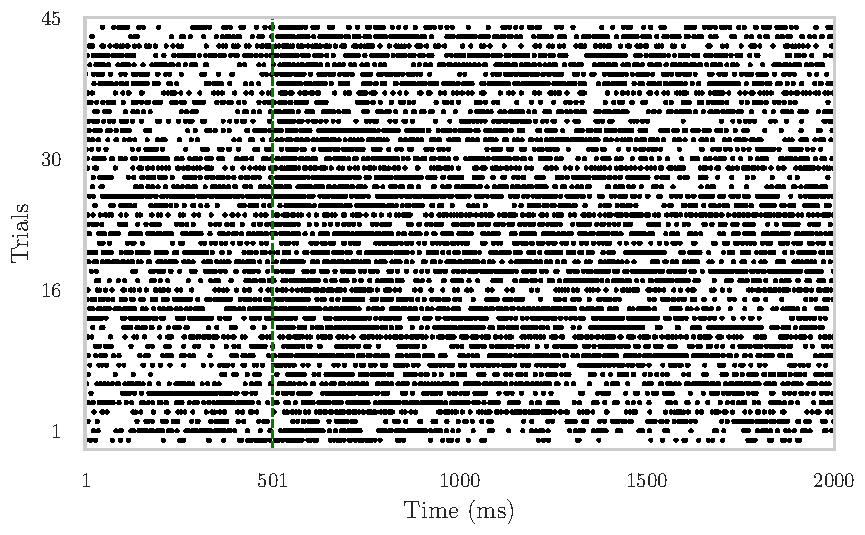
\includegraphics[scale=1]{img/cue_0.pdf}
\end{center}
\caption{Overlaid raster plots of neurons with very excited and unsustained responses. A black dot indicates a spike from at least one of the neurons in the corresponding cluster. The vertical green line indicates cue onset.}\label{cue0-raster}
\end{figure}


\begin{figure}[H]
\begin{center}
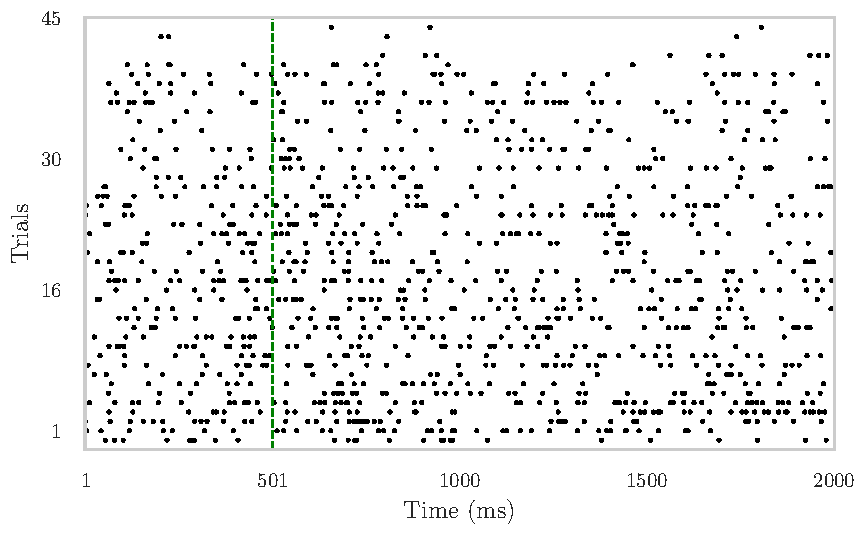
\includegraphics[scale=1]{img/cue_1.pdf}
\end{center}
\caption{Overlaid raster plots of neurons with moderately excited and unsustained responses. A black dot indicates a spike from at least one of the neurons in the corresponding cluster. The vertical green line indicates cue onset.}\label{cue1-raster}
\end{figure}

\begin{figure}[H]
\begin{center}
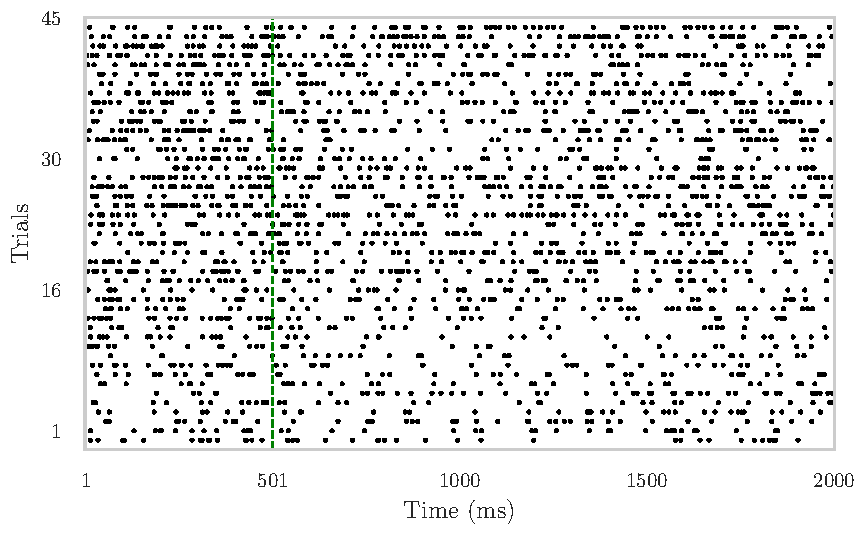
\includegraphics[scale=1]{img/cue_4.pdf}
\end{center}
\caption{Overlaid raster plots of neurons with very inhibited and unsustained responses. A black dot indicates a spike from at least one of the neurons in the corresponding cluster. The vertical green line indicates cue onset.}\label{cue4-raster}
\end{figure}

\begin{figure}[H]
\begin{center}
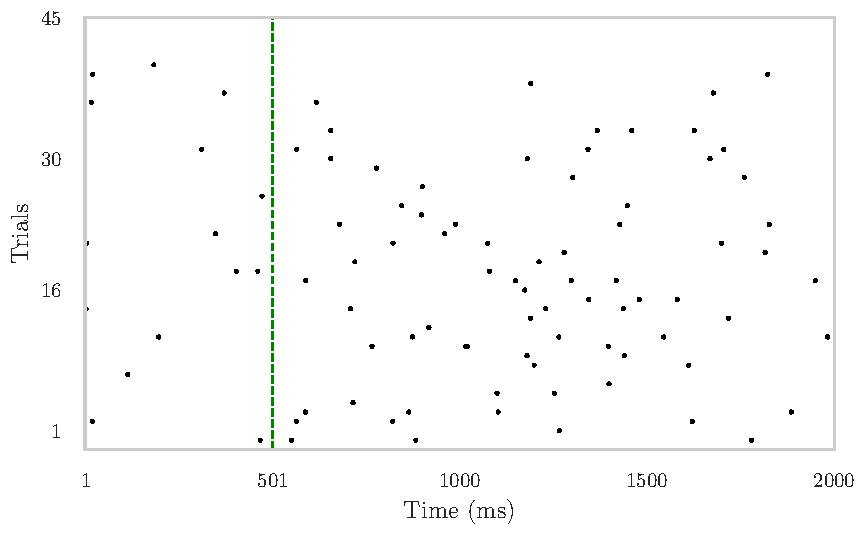
\includegraphics[scale=1]{img/cue_5.pdf}
\end{center}
\caption{Overlaid raster plots of neurons with moderately excited and sustained responses. A black dot indicates a spike from at least one of the neurons in the corresponding cluster. The vertical green line indicates cue onset.}\label{cue5-raster}
\end{figure}

\begin{figure}[H]
\begin{center}
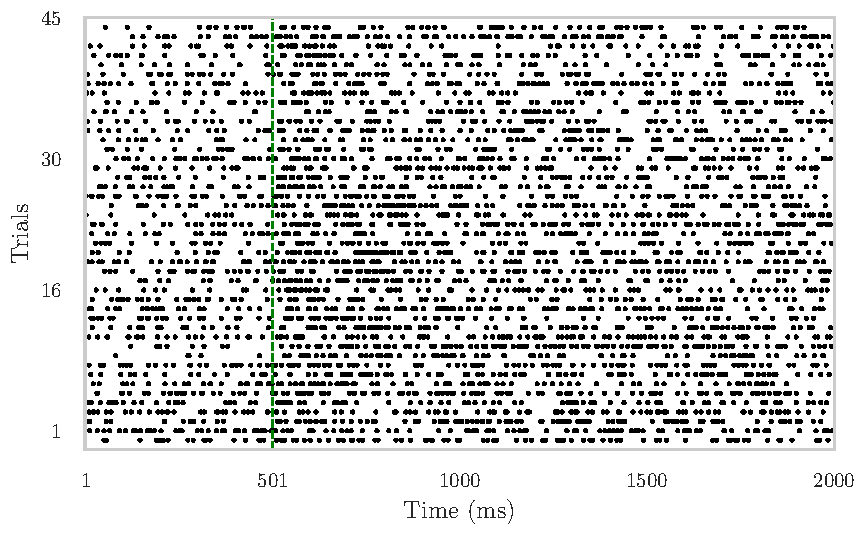
\includegraphics[scale=1]{img/cue_6.pdf}
\end{center}
\caption{Overlaid raster plots of neurons with very excited and unsustained responses. A black dot indicates a spike from at least one of the neurons in the corresponding cluster. The vertical green line indicates cue onset.}\label{cue6-raster}
\end{figure}

\begin{figure}[H]
\begin{center}
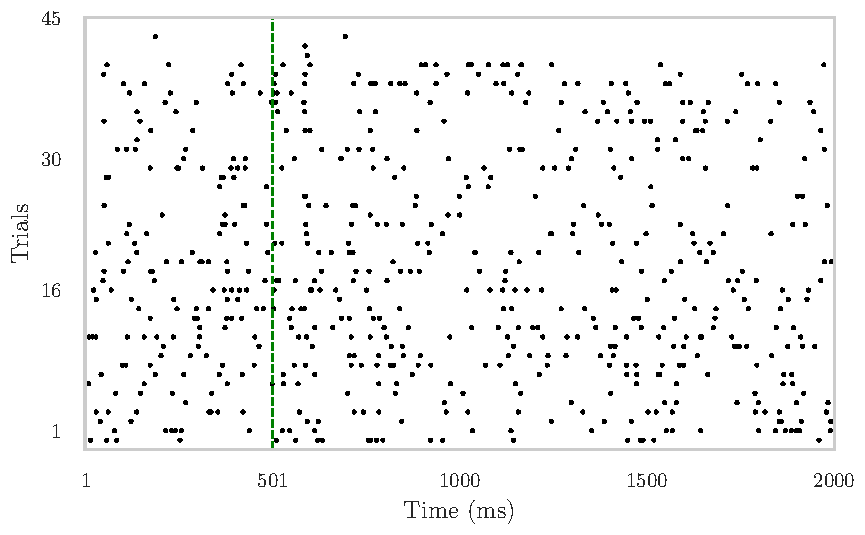
\includegraphics[scale=1]{img/cue_7.pdf}
\end{center}
\caption{Overlaid raster plots of neurons with slightly inhibited and sustained responses. A black dot indicates a spike from at least one of the neurons in the corresponding cluster. The vertical green line indicates cue onset.}\label{cue7-raster}
\end{figure}

\begin{figure}[H]
\begin{center}
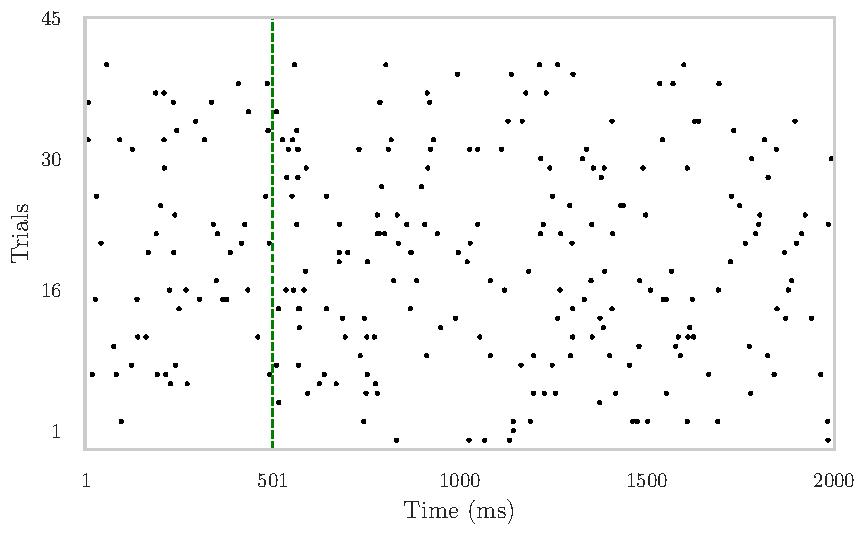
\includegraphics[scale=1]{img/cue_8.pdf}
\end{center}
\caption{Overlaid raster plots of neurons with slightly excited and sustained responses. A black dot indicates a spike from at least one of the neurons in the corresponding cluster. The vertical green line indicates cue onset.}\label{cue8-raster}
\end{figure}

\section{Clustering Shock Responses: How subtle is the effect Figure 6(b) (main text)?}

The fact that Figure~6(b) comprises neurons that are inhibited in response to the shock is not visually apparent. We pick two neurons from the cluster and demonstrate that the shock has an inhibitory, albeit subtle, effect on their response. In particular, we compare the empirical estimate of the rate at all trials $1,\cdots,45$ to an estimate of the rate obtained from the DPnSSM model.
\\
\\
\noindent We compute the empirical rate of events at trial $t$ in units of Hz as $\hat{\lambda}^{\text{emp}}_t = 1000 \cdot y_t^{(n)}/2000$, where the factor of 1000 is to convert the empirical probability estimates to units of Hz.
\\
\\
Suppose the cluster selection method described in the main text selects the samples from Gibbs iteration $i^*$. For a given neuron $n$ with cluster assignment $z^{(n)\langle i^{*}\rangle}$ and parameter $\theta^{(z^{(n)\langle i^{*}\rangle})}$ obtained from hierarchical clustering applied to the co-occurence matrix (please see main text), we use cSMC to generate $S = 64$ samples $x_1^s,\ldots,x_T^s$, where for each $t = 1, \ldots, T$,
\begin{align}
x_t^s \sim p(x_t^{(n)}|z^{(n)\langle i^{*}\rangle},\theta^{(z^{(n)\langle i^{*}\rangle})}, \idx[1] y n, \ldots, \idx[t] y n)
\end{align}
for all $s$.  
We then compute
\begin{equation}
\hat{x}_t = \frac{1}{S} \sum_{s=1}^S x_t^s.
\end{equation}
\noindent Finally, as the DPnSSM estimate of the rate in Hz, we use
\begin{equation}
\hat{\lambda}^{\text{dpnssm}}_t = 1000 \left(\frac{\exp {\hat{x}_t}}{1+  \exp {\hat{x}_t}}\right)
\end{equation}

\noindent Figure~\ref{fig:subtlecue} shows two neurons from the cluster in Figure 6(b). Overall, the empirical rate from each neuron indicates a downward trend, that is accentuated around trial $16$, the trial when shock is delivered. In the DPnSSM, this is captured by the abrupt change in the empirical rate at trial $16$, which indicates the fact that these neurons are inhibited, albeit very subtly so, in response to the shock. In other words, despite the fact this effect is not obvious from the overlaid raster of Figure 6(b), Figure~\ref{fig:subtlecue} indicates that the DPnSSM is able to identify a subtle effect that can be seen in the raw data.


\begin{figure}[H]
\begin{center}
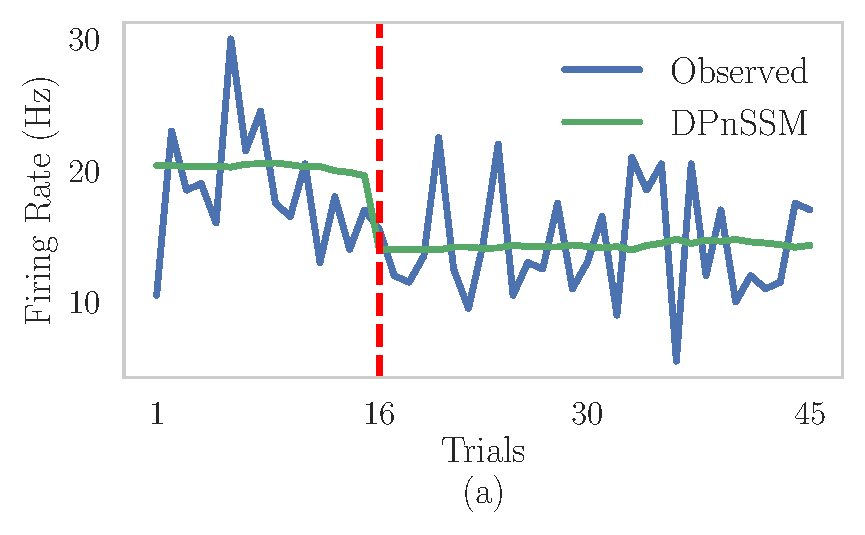
\includegraphics[scale=0.5]{img/state-space-a.pdf}
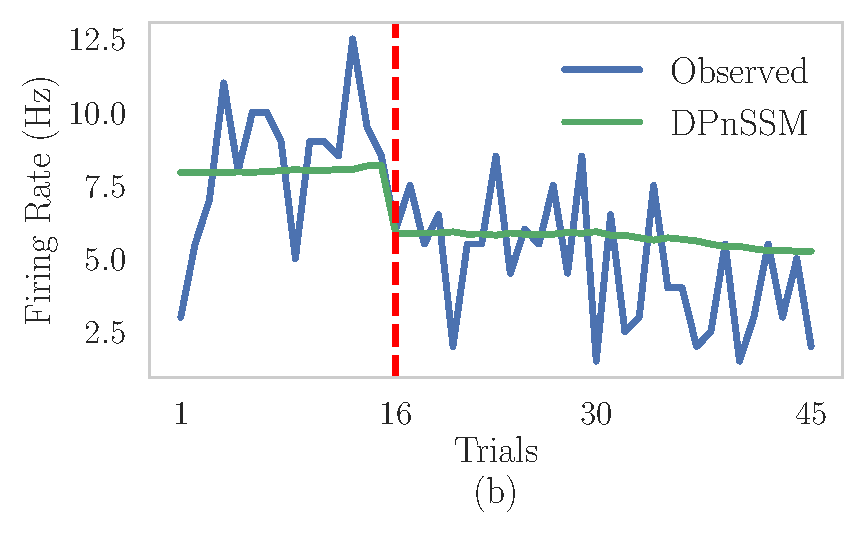
\includegraphics[scale=0.5]{img/state-space-b.pdf}
\end{center}
\caption{Two representative neurons from the cluster corresponding to Figure 6(b).  The DPnSSM state sequence is able to track the overall trend in the observed data and correctly characterize the response to the shock at trial 16 as slightly inhibited.}
\label{fig:subtlecue}
\end{figure}

\bibliographystyle{apalike}
\bibliography{aistats}

\end{document}